\documentclass[letterpaper,twocolumn,10pt]{article}
\usepackage{usenix2019_v3}

\usepackage{microtype}
\usepackage{calc}
\usepackage{tikz}
\usepackage{dblfloatfix}
\usepackage{amsmath}
\usepackage{amssymb}
\usepackage{pifont}
\usepackage{comment}

\usepackage{graphicx}
\usepackage{float}
\usepackage{listings}
\usepackage{booktabs}
\usepackage{paralist}
\usepackage{titlesec}

\newcommand{\tbad}{\makebox[\widthof{\ding{51}}]{\ding{55}}:}
\newcommand{\tgood}{\ding{51}:}

% \titleformat*{\subsection}{\normalsize\bfseries}
% \titleformat*{\subsubsection}{\normalsize\bfseries}
% \titlespacing{\subsection}{0pt}{1ex}{0.5ex}
% \titlespacing{\subsubsection}{0pt}{0.5ex}{0ex}
\lstset{
language=Python,
basicstyle=\small\ttfamily,
keywordstyle=,
stringstyle=\color{red},
frame=tb,
columns=fullflexible,
showstringspaces=false,
belowskip=0pt,
}

\begin{document}
\newcommand{\twosigma}{{[tech company]}}
\newcommand{\githuburl}{[Github url removed]}
\date{}
\title{\Large \bf DRAFT: Direct-style process creation on Linux}
% \author{
% {\rm Spencer Baugh}\\
% Two Sigma
% }
\maketitle
\begin{abstract}
Traditional process creation interfaces,
such as \texttt{fork} and \texttt{spawn},
are complex to use, limited in power, and difficult to abstract over.
We develop a new process creation interface for Linux
which allows a program to create a child process in a non-running state
and initialize the new process by operating on it from the outside.
This method of process creation results in more comprehensible programs, 
has better error handling,
is comparably efficient,
and is more amenable to abstraction.
Our implementation is immediately deployable without kernel modifications on any recent Linux kernel version.
\end{abstract}

\section{Introduction}\label{introduction}
\begin{table*}
\begin{tabular}{l|l|l|l}
% BEGIN RECEIVE ORGTBL compare
 & fork-style & spawn-style & direct-style\\
\hline
Parent process requirements & \tbad Single thread, small memory & \tgood None & \tgood None\\
Programming model & \tbad Complex (returns twice) & \tgood Simple (single call) & \tgood Simple (imperative)\\
Maximally powerful & \tgood Yes, can call any syscall & \tbad No, limited interface & \tgood Yes, can call any syscall\\
Reporting of results & \tbad Requires IPC & \tbad Not fine-grained & \tgood From individual child syscalls\\
Non-inherited attributes & Mutated by code in child & Set by arguments & Mutated by code in parent\\
% END RECEIVE ORGTBL compare
\end{tabular}
\caption{Features of fork-style vs spawn-style vs direct-style}
\label{tab:styles}
\end{table*}
\begin{comment}
#+ORGTBL: SEND compare orgtbl-to-latex :splice t
|                             | fork-style                        | spawn-style                 | direct-style                          |
|-----------------------------+-----------------------------------+-----------------------------+---------------------------------------|
| Parent process requirements | \tbad Single thread, small memory | \tgood None                 | \tgood None                           |
| Programming model           | \tbad Complex (returns twice)     | \tgood Simple (single call) | \tgood Simple (imperative)            |
| Maximally powerful          | \tgood Yes, can call any syscall  | \tbad No, limited interface | \tgood Yes, can call any syscall      |
| Reporting of results        | \tbad Requires IPC                | \tbad Not fine-grained      | \tgood From individual child syscalls |
| Non-inherited attributes    | Mutated by code in child          | Set by arguments            | Mutated by code in parent             |
% $
\end{comment}
The most well-known process creation interface on Linux, and Unix in general, is \texttt{fork}.
When a parent process creates a child process through \texttt{fork} or other fork-style interfaces,
both processes execute concurrently,
and the child process typically inherits all but a few attributes from the parent process\cite{manfork}.
The child process can call arbitrary system calls
to mutate the new process until it reaches the desired state,
typically ultimately calling \texttt{exec}.

A user of \texttt{fork} must think carefully about the characteristics of the process
from which \texttt{fork} is being called.
\texttt{fork} can have poor performance when called from processes with many memory mappings\cite{forkroad}.
This can be mitigated to some degree by using \texttt{vfork} or \texttt{CLONE\_VM},
but those inflict further complexity on the caller\cite{vfork_dangerous}.
Processes which are multi-threaded can encounter deadlocks and other issues if they call \texttt{fork}
\cite{forkroad}\cite{tlpi}\cite{posix_spawn_error_pipe}.
Some thread libraries provide partial mitigations for multi-threading issues\cite{pthread_atfork},
but it's up to user code to make use of those mitigations.

Since the child process runs concurrently with the parent process,
communicating events in the child back to the parent requires some form of IPC\cite{posix_spawn_error_pipe},
adding complexity.
Even the basic interface of \texttt{fork} --- one function call which returns twice --- is unusual;
such functions are generally considered to be complex, advanced topics in other settings
\cite{callcc_fork}\cite{continuations}.

Closely related to \texttt{fork}
are process creation interfaces where the new process is launched running a function of the caller's choice,
which can then call arbitrary system calls to mutate the new process
\cite{clone}\cite{sfork}.
Such interfaces have similar issues as \texttt{fork},
and we class them together as ``fork-style'' interfaces.

On the other hand, in a spawn-style interface,
details about the new process are provided up-front as arguments to some function
which creates the new process all at once.
\texttt{posix\_spawn}\cite{posix_spawn} is a typical example of this style
\cite{chainloading}\cite{create_process}.
Other details, such as security context, are inherited from the parent process\cite{tlpi}\cite{create_process}.
Spawn-style APIs
can be called from any parent process without concerns about memory usage or multi-threading,
when used correctly
\cite{posix_spawn_error_pipe}\cite{forkroad}.

Unlike \texttt{fork}, a spawn-style interface provides an API for process creation
which is independent from normal system calls\cite{spawn_h}\cite{subprocess_run}.
Spawn-style interfaces therefore often lack support for some features,
and they also require learning a new interface distinct from the existing system call API
\cite{posix_spawn_lwn}\cite{tlpi}.
Also, spawn-style interfaces, by their nature as a single call,
don't allow programs to branch on the results of individual modifications to the new process,
and have worse error reporting for such modifications
\cite{posix_spawn}\cite{posix_spawn_error_pipe}.

Table \ref{tab:styles} summarizes the differences between fork-style and spawn-style.
Each has its own advantages and disadvantages.

A few academic operating systems
--- KeyKOS\cite{keykos} and seL4\cite{sel4}, among others\cite{exokernel}\cite{fuchsia}\cite{singularity} ---
use another style of process creation.
We use the new term ``direct-style'' to refer to this,
since we know of no pre-existing generic term for this style of process creation.

In direct-style, a process is created by its parent in a non-running state,
then supplied with various resources,
and then started running once it is fully set up.
In operating systems with true direct-style process creation,
the syscalls that can mutate a process
take explicit arguments to indicate the process on which they should operate\cite{keykos}\cite{sel4}.
In this way, the same syscalls that can mutate a process while it is running
are called by the parent process to mutate the process while it is being set up.

To perform direct-style process creation on Linux,
we need an API where we explicitly specify in which process we want to make a syscall.
This differs from the normal mode of operation on Linux,
where programs making syscalls implicitly operate on the current process.

Our main contribution in this paper is such an API, in the form of the \texttt{rsyscall} library.
\texttt{rsyscall} is a
language-specific, object-capability-model, low-abstraction library for the Linux system call interface,
bypassing libc\cite{capmyths}\cite{robust_composition}.
The \texttt{rsyscall} project is currently focused on supporting Python,
but the library can be ported to other languages.
The examples we show in this paper will be in Python,
but generalize easily.
\texttt{rsyscall} is open source and available from
\githuburl{}.

Unlike typical C libraries such as glibc or musl,
the \texttt{rsyscall} library is organized based on the object-capability model\cite{capmyths}\cite{robust_composition}.
The capability to make syscalls in any specific process is reified as a language object.
If the capability to make syscalls in a specific process is not passed (in some way) to a function,
then that function cannot make syscalls in that process.

Due to this design, an \texttt{rsyscall} program can make use of multiple processes at once,
by manipulating capabilities for multiple processes.
The relevant two types of capabilities for this paper are the initial capability for the ``local'' process,
and capabilities for child processes.
The ``local'' process is the one which hosts the runtime for the running program,
and in which a legacy libc would implicitly make syscalls.
Every \texttt{rsyscall} program starts with the capability for the ``local'' process
and uses it to bootstrap capabilities for other processes.

\lstinputlisting[float,language=Python,label={lst:basic},caption={Create new process, change CWD, and exec}]
{examples/basic/direct.py}
Listing \ref{lst:basic} shows a Python program using \texttt{rsyscall}.
We create a new child process using direct-style \texttt{clone} in the local process \verb|local|.
Here, \texttt{local.clone()} does not create another task running the same user program,
as with the usual \texttt{clone} system call,
but instead returns a capability through which we can control the new child process.
We can then call various syscalls in the child process to mutate it until it reachs the desired state.
In this example,
we call \texttt{chdir} in the child process to change its working directory,
then call \texttt{execv} in the child to execute a new executable.
Calling \texttt{execv} consumes the capability,
releasing the process from our control;
later use of this child process capability will fail with an exception.
The child process can now be monitored using normal Linux child monitoring syscalls,
such as \texttt{waitid}.

These child process capabilities are created and managed in userspace,
by launching new processes running a syscall server,
which receives syscall requests, performs the syscall, and returns the response.
No kernel modifications are required, and \texttt{rsyscall} is immediately deployable on recent Linux kernels.
We discuss the implementation in depth in section \ref{implementation},
and examine several difficult process-creation details.

System calls called in a child process through \texttt{rsyscall}
behave identically to system calls called implicitly in the current process through libc.
A system call returning an error is reported in the standard way for system calls in Python:
An exception is thrown at the point of the call.
User code can branch as normal on the results of system calls,
and implement fallbacks or other error handling logic.

Since we can call any syscall,
we can access any feature available in Linux; we are therefore at least as powerful as \texttt{fork}.
As we'll show in section \ref{examples},
we can in fact use Linux features in ways that are impractical with the usual fork-style or spawn-style interfaces.

Direct-style \texttt{clone} has acceptable performance cost,
and can outperform \texttt{fork} in some cases.
Like a spawn-style interface,
we can call \texttt{clone}
without worse performance in the presence of large memory usage,
and without the possibility of bugs in the presence of multi-threading.
The performance overhead of creating processes with direct-style clone
is comparable to the performance cost of creating processes while inside a Linux namespace.
At \twosigma{}, we've used direct-style process creation
to implement a production library for distributed system deployment.
We evaluate in further detail in section \ref{evaluation}.

In summary, this paper makes the following contributions:
\begin{compactitem}
\item We coin the term ``direct-style process creation''
  to refer to a previously-unnamed style of process creation which is common on academic operating systems.
\item We built \texttt{rsyscall}, a library for the Linux system call interface following the object-capability model.
\item As part of \texttt{rsyscall}, we built the first implementation of direct-style process creation on a Unix-like kernel.
\end{compactitem}
\texttt{rsyscall} is open source and available from \githuburl{}.
\section{Examples}\label{examples}
In this section,
we'll demonstrate direct-style process creation
by using several sophisticated features of Linux processes.
For concision, we assume that we are running with sufficient privileges,
but these examples can all be run without privileges with appropriate use of \verb|CLONE_NEWUSER|
\cite{user_namespaces}\cite{unpriv_fuse}.

In these examples and in this paper,
a single program with a single flow of control is operating across multiple processes.
We'll always describe operations from the perspective of this single synchronous program,
never from the perspective of an individual parent or child process.

These examples are not novel, as such, as they use only conventional Linux system calls;
but implementing them with \texttt{fork} or \verb|posix_spawn| requires substantially more code,
or even a complete change in implementation approach as in section \ref{shared_fd_table}.
We demonstrate this by comparison to fork-style implementations of these examples in section \ref{ease}.

Several of these examples can be implemented by configuring and invoking existing software;
such software effectively provides a specialized spawn-style interface.
But such tools are often inflexible.
For example, a shell allows the creation of pipelines and container systems like Docker allow sandboxing,
but the two are difficult to combine\cite{docker_pipe}.

With improved process creation techniques,
these features can be used directly by programmers
instead of by configuring stand-alone software.
In this way,
individual real-world applications can pick and choose the features that are useful for them,
as we describe in section \ref{realworld}.
\subsection{Abstraction through FD passing}\label{fd_abstraction}
In Linux (and Unix in general),
a program can pass file descriptors (FDs) from the parent process to a child process
by using file descriptor inheritance\cite{tlpi}.
When a process is created, all open file descriptors are copied from the parent process to the child process.
The child process can then make independent use of the file descriptors.
We'll discuss this important feature further in section \ref{inheritance}.

Most resources in Linux are managed through file descriptors,
so this allows the parent process to pass a variety of resources to the child process,
such as files, network connections, pipes, or other resources\cite{ucspi}.
Since the resource is created outside the child process and passed down as an opqaue file descriptor,
the precise details and type of the resource are not available to the child.
This is a form of abstraction,
and so we know ``for free''\cite{theoremsforfree}
that the program running in the child process
will not rely on the details of how the file descriptor was created,
such as the filename that we opened or the hostname to which we connected.

\lstinputlisting[float,language=Python,label={lst:fds},caption={Passing down FDs}]
{examples/fds/direct.py}
In Listing \ref{lst:fds},
we first open a file with read-write permission in the local process.
Then we create a child process,
which inherits all file descriptors from its parent.
We indicate that we want to operate on the child's inherited copy of the file descriptor with \verb|child.inherit_fd|.
\texttt{inherit\_fd} performs no system calls,
it just updates bookkeeping to return a new handle for the inherited file descriptor;
we'll discuss it in more depth in section \ref{inheritance}.
Then we disable \texttt{CLOEXEC} on the child's file descriptor,
which on Linux we can do by clearing the FD flags with \verb|fcntl(fd, F_SETFD, 0)|;
this ensures that the file descriptor will be usable by the new program after we call \texttt{exec}\cite{fcntl}.
Finally, we execute a new program in the child process,
passing the file descriptor number as an argument.
The new program will be able to use the file descriptor we opened through that file descriptor number.
\subsection{Non-shared-memory concurrency}\label{pipe}
Processes run concurrently,
which enables modularity
and allows exploiting the parallelism of the underlying hardware.
Since processes don't share memory,
they can provide a less complex parallel programming environment
than shared-memory thread-based approaches\cite{threads}.

\lstinputlisting[float,language=Python,label={lst:pipe},caption={Creating a concurrent processing pipeline}]
{examples/pipe/direct.py}
In listing \ref{lst:pipe},
we execute a few programs concurrently,
connected by pipes.
The \texttt{source} program generates two outputs, which go to \texttt{video\_sink} and \texttt{audio\_sink}.
We first create two pipes in the local process,
then inherit them down to several child processes using a helper function, \verb|argfd|,
which uses \verb|inherit_fd| and \texttt{fcntl} as described in section \ref{fd_abstraction}.
We call \texttt{execv} in each child process to run the desired programs,
passing some file descriptors as arguments to each.
The whole system of connected processes then runs concurrently.
\subsection{Customization without explicit support}
While ideally all resources would be passed by file descriptor,
traditional Unix has a number of resources that are global,
such as the process identifier space or the mount table,
which cannot be changed on a per-process basis\cite{capsicum}.

In Linux, many global resources have been made process-local
through the namespaces system\cite{lwn_namespaces}.
Like other process-local resources such as the current working directory,
namespaces are typically set up at process creation time.

One key use of namespaces is to implement large-scale container systems such as Docker\cite{lwn_namespaces}.
However, this is far from the only use.
With an adaquate process creation primitive,
namespaces can be used easily on a much smaller scale.

Namespaces, like all process-local resources,
can be used to customize a program's behavior
in ways that were not anticipated at development time
by customizing the environment the process runs in\cite{plan9ns}.
Other system calls such as \texttt{chdir} and \texttt{chroot} can also be used for this,
but namespaces allow new ways of customization\cite{mount_namespaces}.

\lstinputlisting[float,language=Python,label={lst:mount},caption={Overriding absolute path using a mount namespace}]
{examples/mount/direct.py}
One classic form of customization
is overriding files at paths that were hardcoded into a program,
without changing those files for the rest of the system.
In listing \ref{lst:mount},
we create a new child process as normal,
but for the first time,
pass an argument to \texttt{clone}.

\verb|CLONE_NEWNS| causes \texttt{clone} to create the process in a new mount namespace,
which allows us to manipulate the filesystem tree in a way that only this process will see,
using the \texttt{mount} system call\cite{mount_namespaces}\cite{clone}.
We call \texttt{mount}, passing \texttt{MS\_BIND}, to make the file \verb|/home/foo/custom_foo.conf|
appear at the path \verb|/etc/foo.conf|;
this is known as a bind mount\cite{mount}.
Then we execute some program,
which, when it opens \verb|/etc/foo.conf|, will see the contents of our \verb|custom_foo.conf|.
\subsection{Sandboxing}
At process creation time,
we can not only pass resources and customize the process's environment,
we can also deny the process access to resources that it otherwise receives by default.
This is a key part of creating a secure sandbox for potentially malicious code\cite{seccomp}\cite{firejail}\cite{gvisor}.

\lstinputlisting[float,language=Python,label={lst:unmount},caption={Unmount all and run executable via fexec}]
{examples/unmount/direct.py}
In listing \ref{lst:unmount}
we create a new child process,
again in a new mount namespace using \verb|CLONE_NEWNS|.
Since we won't be able to open files or use \texttt{execv} in the child process after the next step,
we open several files in the child up-front.
Then we use \texttt{umount},
passing \texttt{MNT.DETACH} to perform a recursive unmount of the entire filesystem tree,
removing it all from the view of this process.

Then, as in listing \ref{lst:fds}, we prepare to pass \texttt{db\_fd} to the new program by unsetting \texttt{CLOEXC}.
Unlike in listing \ref{lst:fds}, we don't need to call \verb|inherit_fd|,
since the file descriptor was opened directly from the child process.
We then run the executable we opened earlier using \texttt{fexec},
which allows executing a file descriptor,
and pass the database file descriptor number as an argument\cite{execveat}.
Note that this executable must be statically linked,
or it wouldn't work in an empty filesystem namespace
with no libraries to dynamically link against.

By removing the filesystem tree from the view of this process,
we can run this executable with greater confidence
that it won't be able to tamper with the rest of the system.
A sandbox which is truly robust against malicious or compromised programs requires additional steps,
but this is a substantial start\cite{firejail}\cite{gvisor}.
Such a technique can also be used when a full sandbox is not relevant,
to ease reasoning about the behavior of the program being run
and protect against bugs.

Even if the process needs additional resources,
those can be explicitly passed down through file descriptor passing,
as we do here with the database file descriptor.
This allows us to approximate capability-based security\cite{capsicum}.
\subsection{Nested clone and pid namespaces}\label{pidns}
Process-local resources can also be used to control the lifetime of resources used by that process.
Some Linux resources are not automatically cleaned up on process exit;
a poorly coded program may allocate global resources
without ensuring that they will be cleaned up later,
leaving behind unused garbage on the system when it exits.

One resource which is not automatically cleaned up is processes themselves.
If we run a program which itself spawns subprocesses,
those subprocesses may unintentionally leak,
and be left running on the system even after the original program has stopped\cite{caternfork}.

We can use a pid namespace to solve this issue.
The lifetime of all processes in a pid namespace is tied to the first process created in it,
the init process.
When the init process dies,
all other processes in the pid namespace are destroyed\cite{pid_namespaces}.

\lstinputlisting[float,language=Python,label={lst:pidns},caption={Nested clone and pid namespace}]
{examples/pidns/direct.py}
In listing \ref{lst:pidns},
we create a child process which we'll name \texttt{init},
passing \verb|CLONE_NEWPID| to create it in a new pid namespace\cite{clone}.

To create another process in the pid namespace,
we clone again, this time from \texttt{init}.
This is the first example in which we've cloned from one of our child processes;
as normal, this gives us a capability for a new process, a grandchild,
which can be used exactly like a direct child process.
We \texttt{exec} in the grandchild,
and we can monitor the grandchild process from \texttt{init},
just as we would monitor \texttt{init} from its parent process.

The first process in a pid namespace (usually referred to as \texttt{init})
has some special powers and responsibilities\cite{pid_namespaces}.
We can handle these responsibilities ourselves directly from our program,
or we can continue on by \texttt{exec}ing an init daemon in \texttt{init} to handle it for us
\cite{tini}\cite{dumb_init}.

In either case, when \texttt{init} dies,
the pid namespace will be destroyed,
and \texttt{grandchild} will be cleaned up.
\subsection{Shared file descriptor tables}\label{shared_fd_table}
For our final example,
we'll create a child process which shares its file descriptor table with the parent process.
This can be useful for a variety of purposes,
such as accessing resources in other namespaces, or accessing multiple namespaces at once.

Our example will use the Filesystem in Userspace (FUSE) Linux subsystem.
FUSE\cite{fuse} allows a filesystem to be implemented with a userspace program.
Many interesting filesystems\cite{sshfs}\cite{encfs}\cite{mp3fs} have been implemented using FUSE,
representing a variety of resources as files.

For improved modularity, we might want to mount and use a FUSE filesystem in our program,
in a way that no other process can see it,
without entering a new namespace ourselves.
We can do this by creating a child process that shares its file descriptor table with the parent process.

\lstinputlisting[float,language=Python,label={lst:fuse},caption={Shared file descriptor tables}]
{examples/fuse/direct.py}
In listing \ref{lst:fuse},
we first create a child process \verb|ns_child| in a new mount namespace with \verb|CLONE_NEWNS|,
and this time also pass \verb|CLONE_FILES|,
which causes the file descriptor table to be shared between the parent process and the child process\cite{clone}.
We create another child from \verb|ns_child|
and use it to \texttt{exec} a FUSE filesystem,
which will appear only in the mount namespace of \verb|ns_child| and its descendents.
Then we can open FUSE files in \verb|ns_child|
and use those files in \texttt{local},
through the shared file descriptor table.
We call \texttt{use\_fd} which, like \texttt{inherit\_fd},
updates bookkeeping to create a new handle for the file descriptor existing in the shared fd table;
we'll discuss \texttt{use\_fd} in section \ref{inheritance}.

File descriptor passing over a Unix domain socket
can allow similar behavior without sharing the file descriptor table,
but is substantially more complex\cite{scm_rights}.
Nevertheless, for fork-style and spawn-style process creation,
file descriptor passing over a Unix domain socket
is our only option to implement this kind of sharing.
\section{Implementation}\label{implementation}
In this section, we'll give a brief overview of the implementation of \texttt{rsyscall},
and then focus on implementation issues specific to process creation.

\texttt{rsyscall} can be conceptually divided in two parts:
the basic syscall primitive,
and a language-specific library built on top.
The Python language-specific library has already been demonstrated above.
Such libraries only need to be able to call syscalls and explicitly specify a process in some way;
they are, for the most part, agnostic to how the syscall primitive is implemented.
The syscall primitive takes a syscall number, and some number of register-sized integer arguments,
and arranges to call that syscall in the specified process,
returning the response as a single register-sized integer.

When making a syscall in the local process, the syscall is performed normally,
directly on the local thread, as one might expect.

When making a syscall in another process,
\texttt{rsyscall}'s default userspace cross-process syscall primitive sends the syscall request
to a userspace ``syscall server'' running in the target process,
which performs the syscall and sends the response back.
Communication to the syscall server happens over file descriptors,
typically a pair of pipes.
The syscall server runs on the main and only thread of the target process,
and is the only userspace code running in an rsyscall-controlled child process;
when not executing a syscall or writing out the response,
an rsyscall-controlled child process spends all its time blocked in \texttt{read},
waiting for new syscall requests.

We use file descriptors for transport of data rather than shared memory
to support straightforward integration with existing event loops;
this is a key design constraint.
While we only show synchronous programs in this paper,
calling a syscall in another process may block at any time,
and a complex program will likely have other requests to service concurrently.
Even a relatively simple program may want to monitor multiple child processes at a time.
To support this,
our implementation fully supports asynchronous usage with a user-provided event loop,
including Python \texttt{async/await} coroutine support\cite{python_coroutines}.

We have chosen to implement our cross-process syscall primitive in userspace,
rather than immediately implementing this in the kernel,
to aid deployability
and to allow fast iteration while developing userspace code using these features.
In the past, attempts to upstream kernel support for novel features without extensive userspace usage
have had a poor reception in the Linux kernel community\cite{lwn_checkpoint}\cite{first_class_address_space}.
We believe proving viability in userspace first will be better in the long term.

\texttt{ptrace} already provides an in-kernel way to perform arbitrary actions on a target process,
including system calls,
but is not suitable for us\cite{ptrace}.
As we discuss in section \ref{related}, a number of systems, such as \texttt{gdb} and \texttt{strace},
use \texttt{ptrace} to implement debuggers.
But multiple processes cannot use \texttt{ptrace} on a single target process at the same time;
thus, if we used \texttt{ptrace} to implement \texttt{rsyscall},
such debugging tools would not work on \texttt{rsyscall}-controlled processes,
which is an unacceptable limitation for a general-purpose utility.

Many syscalls either take or return pointers to memory,
and require the caller to read or write that memory to provide arguments or receive results.
Therefore, an \texttt{rsyscall} library needs a way to access memory in the target process.

The most simple way to access memory is for the local process to be in the same address space as the target process.
This is the case most of the time; we pass \verb|CLONE_VM| to \texttt{clone} by default
in the \texttt{rsyscall} wrapper for \texttt{clone}.

Sometimes, the target process may be in another address space;
for example, if the target process is at a different privilege level,
we will want it to be in a different address space for security reasons\cite{vfork_dangerous}.
There are a number of available techniques in that scenario;
we choose to copy memory over a pair of pipes,
again using file descriptors for the sake of easy event loop integration.
\subsection{\texttt{clone}}\label{clone}
Now that we've established the basic implementation details of \texttt{rsyscall},
we'll consider specific issues related to process creation and initialization.

Besides \texttt{clone}, \texttt{vfork} and \texttt{fork} also create processes,
but they are not suitable for flexible direct-style process creation.
\texttt{vfork}\cite{vfork} suspends execution of the parent process
while waiting for the child process to exit or call \texttt{execve},
which is immediately unsuitable.
\texttt{fork} lacks many features which are restricted to \texttt{clone}.
For example, with \texttt{fork},
we could not create child processes which share the parent's address space,
which would complicate memory access.

The raw \texttt{clone} system call creates a new process
which immediately starts executing at the next instruction after the syscall instruction,
in parallel with the parent process,
with its registers in generally the same state as the parent process.

\texttt{clone} lets us change the stack for the new process.
We can use this to make the new process call an arbitrary function,
by storing its address on the new stack.
Further arguments can also be passed on the stack,
with the aid of a trampoline to match C calling conventions if necessary.

We use this to create processes running the syscall server.
After this,
the parent process can begin to call system calls in the child process.
Most system calls work as normal;
the new child process can be modified freely through \texttt{chdir}, \texttt{dup2}, and other system calls.
From the system calls related to process creation,
only \texttt{execve} needs substantial further attention.
\subsection{\texttt{exec}}\label{execve}
\texttt{execve} is unusual and requires careful design,
because when it is successful, it does not return.
We need a way to determine if \texttt{execve} is successful;
naively waiting for a response to the syscall request may leave us waiting forever.

There is a traditional technique used with \texttt{fork}
to detect a successful \texttt{execve} using a pipe,
which unfortunately won't work for us.
With this technique, the parent process creates a pipe before forking,
ensures both ends are marked \texttt{CLOEXEC},
performs the \texttt{fork},
closes the write end of the pipe,
and \texttt{read}s the read end of the pipe.
The child process either successfully calls \texttt{execve} or exits;
either way, the last copy of the write end of the pipe will be closed,
which causes the \texttt{read} in the parent process to return EOF.
The parent can then check that the child process hasn't exited;
if the child hasn't exited, then it must have successfully called exec.

This trick works with \texttt{fork},
but it's not general enough to work with \texttt{clone}.
Child processes can be created with the \verb|CLONE_FILES| flag passed to \texttt{clone},
which causes the parent process and child process to share a single fd table;
we showed an example of this in section \ref{shared_fd_table}.
This means that when the parent process closes the write end of the pipe,
it will also be closed in the child process,
and the read end of the pipe will immediately return EOF,
before the child has called \texttt{execve} or exited.

Fortunately, there is an alternative solution, which does work with \verb|CLONE_FILES|.
\texttt{clone} has an argument, \texttt{ctid}, which specifies a memory address\cite{clone}.
If the \verb|CLONE_CHILD_CLEARTID| flag is set,
then when the child exits or successfully calls \texttt{exec},
the kernel will set \texttt{ctid} to zero and then,
crucially, perform a futex wakeup on it.

Futexes are usually used for the implementation of userspace shared-memory synchronization constructs\cite{futex},
but the relevant detail for us here is that we can wait on an address
until a futex wakeup is performed on that address.
This means we can wait on \texttt{ctid} until the futex wakeup is performed,
and in this way receive a notification when the child process has exited or successfully called \texttt{exec}.

A process can only wait on one futex at a time;
to monitor multiple futexes from a single event loop,
we need to create a dedicated child process for each futex we want to wait on,
and have this child process exit when the futex has a wakeup.
We can then monitor these child processes from an event loop using standard techniques\cite{signalfd}\cite{pidfd}.

So, we pass \texttt{ctid} whenever we call \texttt{clone},
and set up a process to wait on that futex.
Then, when we call any syscall,
we wait for either the syscall to return an error or the futex process to exit,
whichever comes first.
For other syscalls, either result will indicate that the syscall fails,
but for \texttt{execve}, if the futex process exits,
without the child process itself exiting,
then we know that the child has successfully completed the \texttt{execve} call.

If the futex process and child process both exit,
it's ambiguous whether the child process successfully called \texttt{execve};
this ambiguity is unfortunate, but it is also present in the pipe-based approach.
This ambiguous situation will only happen
if the child receives a fatal signal while calling \texttt{execve},
which we believe will be rare.

Some other Unix-like systems natively provide the ability to wait for a child's \texttt{execve}\cite{freebsd_kqueue};
our implementation would be simplified, and the ambiguity eliminated,
if we had this ability on Linux.
One approach would be to add a new \texttt{clone} flag to
opt-in to receiving \texttt{WEXECED} events through \texttt{waitid}.
A new \texttt{waitid} flag alone is not sufficient,
since, to integrate this feature into an event loop,
it's necessary to receive \texttt{SIGCHLD} signals or readability notifications on a pidfd
when the \texttt{WEXECED} event happens.
\subsection{Handling file descriptors}\label{fd_handles}
In Linux, there are many types of resources maintained inside the kernel
which are referred to by identifiers which are valid only within a certain context.
For example, file descriptors are referred to by file descriptor numbers
which are valid only in a certain file descriptor table;
memory and memory mappings are referred to by memory addresses
which are valid only in a certain address space;
the same pattern is followed for a number of other resources\cite{tlpi}.
Each process has one file descriptor table, one address space, and one of each of the other contexts.
Two or more processes can share individual contexts;
for example, two processes might share an address space, but not a file descriptor table.

The core issues here are the same for all such resources,
so we'll focus on file descriptors.
For concision and clarity, we'll abbreviate ``file descriptor'' as ``FD'' in this section.

A typical POSIX program operates within only one process,
and so only needs to concern itself with one of each kind of context.
To identify and operate on an FD, it can use just an FD number,
which is valid within the global implicit process's FD table.
That's sufficient to make syscalls involving that FD.

A program using \texttt{rsyscall}, however,
operates in multiple processes,
and has to deal with resources across multiple contexts.
To identify an FD,
it needs not just a FD number,
but also some kind of identifier for an FD table.
To then operate on that FD,
it needs a capability for a process with that FD table,
so that it can make syscalls in that process.

To manage this, we add a new concept alongside FD, FD number, and FD table:
The FD handle.
An FD handle is a pair of an FD number and a process capability.
This both precisely identifies an FD, and allows operating on it.
We say an FD handle is associated with a process
if that FD handle contains that process capability.

All system calls which would otherwise return FD numbers or take FD numbers as an argument,
now instead return FD handles or take FD handles as an argument.
For convenience, as shown in section \ref{examples} for \texttt{fcntl},
helper methods on the FD handle object are provided for many system calls dealing with a single FD;
these methods simply call the corresponding underlying system call
using the process capability contained in the FD handle.

In this way, we can work with FDs without the ambiguity of dealing with raw FD numbers in a multi-process context.
\subsubsection{File descriptor inheritance and table sharing}\label{inheritance}
The picture is complicated by the need to support some FD behaviors which implicitly cross between processes;
specifically, FD inheritance and FD table sharing.

FD inheritance is a behavior exhibited by \texttt{clone} (without \verb|CLONE_FILES|) and by \texttt{fork}.
When these system calls are called,
they create a new child process with a new FD table.
The new FD table contains copies of all the FDs existing in the parent process's FD table at the time of the system call,
at the same FD numbers.
We show examples of this in sections \ref{fd_abstraction} and \ref{pipe}.

FD table sharing occurs when \texttt{clone} \textit{with} \texttt{CLONE\_FILES} is called;
this creates a new child process that shares its FD table with its parent.
As a result, either process can operate on any FD in the table,
through the same FD numbers.
We show an example of this in section \ref{shared_fd_table}.

These behaviors are unusual in that they operate on all open FDs at once.
There are other ways to pass FDs between processes,
such as \texttt{SCM\_RIGHTS}\cite{scm_rights},
but those interfaces operate on individual FDs through explicit system call arguments and return values.
In those interfaces,
one or more FDs are explicitly passed as arguments to a system call in one process,
and one or more FDs are returned from another system call in another process.
This differs from FD inheritance and FD table sharing, which happen for all FDs, implicitly;
these behavior must be dealt with differently to be fully supported.

\texttt{rsyscall} supports both behaviors in the same way:
by allowing us to create new FD handles
referring to the already-open FDs created by FD inheritance or FD table sharing.
By creating new FD handles associated with new processes, we can call syscalls in those processes on those FDs.

\texttt{rsyscall} provides two functions
\texttt{inherit\_fd} (used in listings \ref{lst:fds} and \ref{lst:pipe})
and \texttt{use\_fd} (used in listing \ref{lst:fuse}), which support FD inheritance and FD table sharing, respectively.
Both functions take as arguments a process capability $A$ and an FD handle $F$ associated with some other process $B$,
and return a new FD handle associated with process $A$.

For \texttt{inherit\_fd},
the returned handle has the same FD number as $F$,
and refers to the copy of $F$'s FD that was inherited at process creation time.
\texttt{inherit\_fd} will fail if $B$ is not $A$'s parent process,
or if $F$ was not open at the time $A$ was created.

For \texttt{use\_fd},
the returned handle again has the same FD number as $F$,
and refers to the \textit{same} FD as $F$, through the shared FD table.
\texttt{use\_fd} will fail if $A$ and $B$ don't share the same FD table.

\texttt{rsyscall}'s support for these behaviors is intended to expose the native functionality of the Linux kernel,
while still being relatively straightforward to use.
In this way,
we hope to ensure that direct-style process creation with \texttt{rsyscall}
supports everything that the underlying Linux system call interface can support.
\section{Evaluation}\label{evaluation}
Our goal is a powerful approach to process creation that is easy to use correctly.
Performance of our implementation is secondary,
but the overhead of our implementation relative to alternative approaches
must be low.

We evaluate the degree to which we meet this goal by answering the following questions:
\begin{compactitem}
\item
  Does direct-style process creation on Linux allow for simpler programs than the alternatives?
  We compare implementations of similar functionality using both direct-style and fork-style in \ref{ease},
  and find substantial benefits for direct-style.
\item
  Does our \texttt{rsyscall}-based direct-style process creation interface
  have acceptable performance overhead relative to the alternatives?
  We evaluate a number of microbenchmarks in \ref{subprocess_bench},
  and find an acceptable level of overhead.
\item
  Does direct-style process creation perform well in the ``real world''?
  We discuss our positive experience with using direct-style process creation at \twosigma{} in \ref{realworld}.
\end{compactitem}
\subsection{Ease of programming with direct-style}\label{ease}
\begin{table}
\begin{tabular}{rrrr}
\hline
Name & Listing & Direct-style & Fork-style \\
\hline
basic & \ref{lst:basic} & 3 & 14 \\
fds & \ref{lst:fds} & 6 & 16 \\
pipe & \ref{lst:pipe} & 17 & 49 \\
mount & \ref{lst:mount} & 4 & 15 \\
unmount & \ref{lst:unmount} & 7 & 18 \\
pidns & \ref{lst:pidns} & 3 & 23 \\
fuse & \ref{lst:fuse} & 6 & 27 \\
\hline
\end{tabular}

\caption{Line counts with direct-style vs fork-style}
\label{tab:ease}
\end{table}
Does direct-style process creation on Linux allow for simpler programs than the alternatives?
To answer this, we compare the direct-style examples shown in section \ref{examples}
to programs with the same behavior implemented in fork-style.

Most of the examples cannot be implemented with typical Linux spawn-style interfaces such as \verb|posix_spawn|,
so we compare only to fork-style.

The line counts of the direct-style and fork-style implementations are listed in table \ref{tab:ease}.
Direct-style consistently takes under half the lines to express the same functionality.

\lstinputlisting[float,language=Python,label={basic_fork},caption={Fork-style: Creating a new process, changing CWD, and execing}]
{examples/basic/fork.py}
Listing \ref{basic_fork} shows one of our fork-style implementations,
corresponding to the direct-style implementation in listing \ref{lst:basic}.

In our fork-style implementations,
we assume substantial infrastructure is available to make fork-style simpler;
despite this, fork-style implementations are still significantly more verbose than direct-style.
We assume the existence of a robust IPC system,
with communication channels set up automatically between the parent process and the child process,
with an already-defined protocol which can cover all errors from all system calls.

The main source of additional code in fork-style implementations
is reporting errors back to the main program using IPC.
This pattern is common in complex usage of \texttt{fork}\cite{posix_spawn_error_pipe}\cite{python_subprocess_errpipe}.
Many users of \texttt{fork} avoid complex IPC
by encoding a subset of the error information into the exit code of the child process
when an error is encountered during child setup.
Such an approach removes the need for IPC,
but still requires similar code for catching errors, encoding them into the exit code,
and detecting the error in the parent process by decoding the exit code.

Direct-style does not require any extra work to report errors from the child process;
errors are reported just like any other system call.
This is the main immediately visible simplification of using direct-style process creation.

It is possible to build an abstracted wrapper for fork-style process creation
which abstracts away this error reporting code.
We have built several such wrappers\cite{sfork},
but have ultimately discarded them in favor of direct-style process creation.

We found that such wrappers, besides their complexity,
don't provide any fundamental improvement
for the issue of communication between the concurrently executing child process and parent process.
As a result, while such wrappers can remove some boilerplate in easy cases,
they remain complex in difficult cases like in sections \ref{pidns} and \ref{shared_fd_table},
which rely on a single program being able to coordinate multiple processes.
We believe only direct-style process creation is able to easily express such functionality.

Direct-style also removes the need to be concerned about the state of the calling process,
though this simplification is not immediately visible in a small example.
The fork-style implementations may break if there are multiple threads in the calling process,
and may be slow if the calling process has large amounts of memory mapped, as we'll see in section \ref{subprocess_bench}.
The direct-style implementations do not have these limitations.
\subsection{Microbenchmark results}\label{subprocess_bench}
\subsubsection{Basic process creation}
\begin{figure}[h!]
\centering
 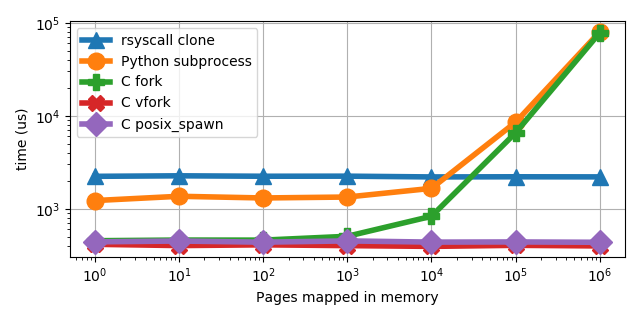
\includegraphics[width=0.5\textwidth]{subprocess_bench}
 \caption{Python spawn-style vs direct-style performance under varying memory usage}
 \label{fig:subprocess_bench}
\end{figure}
We evaluate a simple process creation workload:
create a child process, exec the \texttt{true} binary, and wait for it to exit.
We implement this using Python \texttt{rsyscall} direct-style \texttt{clone},
the Python standard library's \texttt{subprocess.run} (which is implemented primarily with \texttt{fork}),
\texttt{fork} from C,
\texttt{vfork} from C,
and \texttt{posix\_spawn} from C.
We run on CPython 3.7.7, glibc 2.30, Linux 4.19.93,
pinned to an isolated single core on an Intel i9-9900K CPU at standard clock speed,
with 60GB of RAM.
We vary the amount of anonymous memory mapped in the parent process
to demonstrate how each implementation scales with memory usage.
The results are summarized in figure \ref{fig:subprocess_bench}.

Our true baseline for performance is the Python standard library's \texttt{subprocess.run};
this takes an average of 1.4 milliseconds at low memory usage,
while \texttt{rsyscall}'s \texttt{clone} takes an average of 2.2 milliseconds at any memory usage.
As expected, the \texttt{fork}-based implementations scale linearly with memory usage,
and the C implementations vastly outperform the Python implementations.
glibc's \texttt{posix\_spawn} takes an average of 440 microseconds to start a process,
and \texttt{vfork} takes 400 microseconds,
regardless of the memory usage of the calling process,

We perform another microbenchmark to evaluate the overhead of performing additional modifications of the child process.
We call \texttt{getpid} from Python
in both the child process and the parent process on the same benchmark setup.
The average time per \texttt{getpid} call is
3 microseconds when called in the parent process without going through \texttt{rsyscall},
and 561 miroseconds when called through \texttt{rsyscall} in the child process.
The difference, 558 microseconds,
is the amount of overhead incurred
for each child process setup system call performed through \texttt{rsyscall}.

These slowdowns in process creation and modification are substantial,
but we found that this overhead is acceptable in practice.
Process creation in Python is already slow, taking milliseconds of time,
so it is not expected to be on the fast path.
In that context, \texttt{rsyscall} has a reasonable cost compared to \texttt{subprocess.run},
and avoids the bad scaling of \texttt{fork} which might be unexpected by the naive programmer.

Furthermore, as we'll discuss in section \ref{realworld},
we've found that the greater expressivity of direct-style
provides for programs that are more efficient on a large scale,
which makes up for the performance cost in micro-benchmarks.
We've also found that, for many interesting applications,
the performance overhead of direct-style process creation (or Python, for that matter)
is dwarfed by the execution time of the native-code programs we ultimately run.

As a result, though implementations in native code and in the kernel would likely remove most of this overhead,
we have chosen to not invest effort into optimizing process creation at this micro-level,
to preserve implementation simplicity;
such optimization is reserved for future work.
\subsubsection{Nested processes, \texttt{CLONE} flags}\label{clone_bench}
\begin{figure}
\centering
 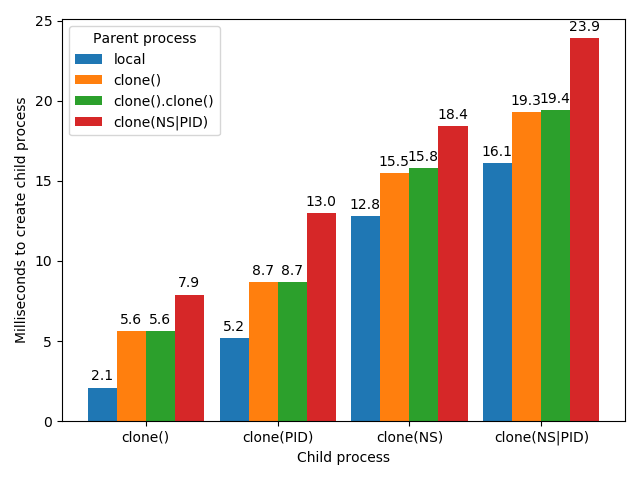
\includegraphics[width=0.5\textwidth]{clone_bench}
 \caption{Time to create different processes from \texttt{rsyscall}, by variety of parent process and child process}
 \label{fig:clone_bench}
\end{figure}
As demonstrated in sections \ref{pidns} and \ref{shared_fd_table},
\texttt{rsyscall} supports nested operation.
That is, we can spawn a child from one of our children;
this can impact performance.
\texttt{clone} also supports specifying a variety of flags to create new namespaces when creating the child,
which can also impact performance.

We've benchmarked process creation using the same simple process creation workload as section \ref{subprocess_bench},
performed through \texttt{rsyscall} from a variety of parent processes:
the local process,
a child (created with \texttt{clone()}),
a grandchild (created with \texttt{clone().clone()}),
or a child in a different namespace (created with \verb=clone(CLONE_NEWNS|CLONE_NEWPID)=).
We've also specified different combinations of flags for the child process being created in the benchmark.
We don't include the Python standard library in these benchmarks
as there's no way to create nested child processes or specify \texttt{CLONE} flags in the Python standard library.
The results are in figure \ref{fig:clone_bench}.

Process creation in a child has a significant performance impact,
primarily because of the overhead of performing syscalls in a child.
Performance of process creation in a grandchild is the same as in a child,
because there is no additional overhead for syscalls in a grandchild relative to a child.
Benchmarking \texttt{getpid} in a grandchild
confirms that the average time per \texttt{getpid} call is still 561 microseconds on our benchmark setup.

The use of namespaces also has a significant impact,
both when the parent process is in a namespace, and when the child process is created in a namespace.
We perform the benchmark with no clone flags, and with the common clone flags
\verb|CLONE_NEWNS| and \verb|CLONE_NEWPID|, first on their own and then together.
This benchmark essentially measures the performance of the Linux namespaces system, not the work in this paper,
but it is illustrative to compare it to the performance of \texttt{rsyscall}.

Note that the cost of creating a new child process from a parent process that is already inside a namespace
(the difference between the \texttt{clone()} and \texttt{clone(NS|PID)} parent processes)
is around 2 milliseconds, comparable to the cost of running with \texttt{rsyscall}.
Note also that the overhead of creating a new process inside a new namespace
(the difference between the \texttt{clone()} and \texttt{clone(NS|PID)} child processes)
is around 15 milliseconds; subtantially greater than the overhead of \texttt{rsyscall}.
As namespaces are widely used,
this suggests our overhead is acceptable.
\subsection{Usage in the real world}\label{realworld}
At \twosigma{} we have used \texttt{rsyscall} and direct-style process creation
to implement an internal distributed system deployment library, written in Python,
which we'll refer to here as Toplevel.
Toplevel is in use in production,
and is extensively used as part of testing and development.
Toplevel consists of a collection of functions and modules
for each component in our system,
which start up components using direct-style process creation,
all from a single Python parent process.

One of the major benefits of direct-style process creation has been easy use of file descriptor inheritance.
Our experience has been that with fork-style or spawn-style interfaces,
file descriptor logic must ultimately be centralized,
while with direct-style,
file descriptors in a new process can be built up over time,
simplifying the implementation.
We've found that even programmers without substantial prior experience with Unix programming
are able to use file descriptor passing as a normal feature of their development process with relative ease,
writing code to support new programs and passing down file descriptors to those programs without issue.

Easy file descriptor passing has, in turn, allowed us to heavily use socket activation techniques
to start up services in parallel,
substantially speeding up system startup\cite{socketactivation}.
We are able to bootstrap connections over our internal shared memory transports
over pre-created, passed-down file descriptors,
and our management interfaces listen on passed-down sockets;
this allows starting up services in parallel, rather than in dependency order.
Benchmarking a representative example built with an old library
and its equivalent built with Toplevel,
the old example took an average of 221 seconds to run,
mostly spent in system startup,
while the new example takes an average of 16 seconds.

Easy file descriptor inheritance has also allowed us to treat file descriptors as a uniform interface in Toplevel.
We pass around file descriptors freely inside Toplevel.
This uniform interface allows us to flexibly swap implementations between in-process and out-of-process,
allowing us to decide on a case-by-case basis
whether we prefer the flexibility of an in-process Python implementation,
or the performance of a native code implementation running in a child process.

We've also made use of namespaces,
chiefly user namespaces and pid namespaces.
For legacy applications which directly start subprocesses,
we prevent process leaking with a pid namespace.
This is part of a strategy of noninterference and cleanup
that ensures that multiple users of Toplevel
can coexist simultaneously on the same host,
even if running the same system.

Toplevel also makes uses of other features of \texttt{rsyscall} which are not covered in this paper,
and will be covered in future work.
These include the ability to operate on remote hosts through capabilities for remote processes,
and the ability to perform system calls in parallel across a pool of processes.
These have significant synergy with direct-style process creation
in forming an overall powerful system.

All this has allowed us to run our systems in a much more dynamic way than before.
We can freely start up arbitrary subsets of our systems on-demand,
spread across one or more hosts,
for development, testing, or production,
regardless of the configuration of that host,
without worrying about interference between instances,
and without a dependency on any external privileged services,
such as container runtimes.
This has become a key part of our development workflow.
\section{Related work}\label{related_work}
\subsection{Direct-style process creation}
Baumann (2019) briefly suggests cross-process operations as a possible replacement for \texttt{fork} on Unix,
positing many of the same advantages we find in practice\cite{forkroad}.
Our work, though developed independently,
is in many ways an elaboration on and implementation of that idea.

As we discuss in section \ref{introduction},
many academic operating systems have direct-style process creation.
We are not aware of any other instances of direct-style process creation in a Unix-like environment.

The closest related work known to us
is efforts to build Unix compatibility environments
on academic operating systems which natively use direct-style process creation;
examples include Exokernel and Fuchsia\cite{exokernel}\cite{fuchsia_libc}.
Such compatibility environments could be bypassed to perform direct-style process creation
using the underlying primitives,
but regular Unix system calls could not be used to create new Unix processes in a direct-style way
in such an environment.
\subsection{Remote system calls}\label{related}
Many Unix-based systems have features described as ``remote system calls''.
Most such systems do not allow a single program to manipulate multiple processes;
rather, a program implicitly makes system calls in a single remote process
which is distinct from the process the program's code runs in.
Those systems that do allow manipulating multiple processes
are generally oriented towards debugging and introspection,
and are unsuitable for a general purpose system.

% probably we should rework this whole section to say "X and Y, among other systems, do Z."
HTCondor\cite{condor} and Popcorn\cite{popcorn}, among others,
use system call forwarding to implement migration between hosts in a computing cluster.
In these systems, processes can be live-migrated between hosts;
when this occurs, the system will transparently forward IO-related system calls
back to the original host.

gvisor\cite{gvisor} and ViewOS\cite{viewos}, among others,
use system call interception as a means of virtualization.
In these systems,
system calls made in one process are intercepted and forwarded to another process,
which performs the specified system call and returns the results back to the original process.

Many other systems have unusual system call invocation patterns,
such as enclave systems like SCONE\cite{scone}\cite{eleos}
or systems for exception-less system calls like FlexSC\cite{flexsc}.
In these systems, for a variety of reasons,
a system call in one process is not evaluated by directly entering the kernel,
but instead is sent to some other process or thread to be evaluated,
and the results received from that process or thread.

A number of debugging or instrospection systems have the ability to perform or monitor system calls in other processes,
typically using ptrace.
Systems like gdb and CRIU
retrieve information about the target process by forcing it to call various system calls to dump information.
These systems typicaly use \texttt{ptrace},
which can be used by a single ptracer process to operate on multiple target processes at once.
Unfortunately, as discussed in section \ref{implementation},
multiple ptracer processes cannot use \texttt{ptrace} on a single target process simultaneously,
which means only one of these systems can be used at a time.

% maybe mention the notion of a formal interface definition for the linux syscall interface
% that might go in future work even.
% yeah it's not yet something developed.
% a formal interface definition so that remote system calls can be employed without building a new system every time.
\subsection{Process capabilities}
Many capability-oriented operating systems, such as KeyKOS\cite{keykos}, seL4\cite{sel4}, and others\cite{fuchsia},
have process capabilities which allow one process to operate on another process.
These systems are our main inspiration for this work.

On several Unix systems,
Capsicum\cite{capsicum} provides something called process descriptors,
which is a file descriptor handle for a process.
A similar feature has been recently added to Linux in the form of the pidfd API\cite{pidfd}.
These notions of process capability are quite limited, however;
pidfds and process descriptors only allow sending signals to a process or waiting for its death,
rather than exercising full control over the process.
\subsection{Capability-secure libc replacements}
Capsicum\cite{capsicum} provides a set of system calls
which can be used to provide a capability-secure sandbox.
Latter efforts\cite{oblivious}, including CloudABI\cite{cloudabi} and WASI\cite{wasi},
developed this into a partial or full replacement for a POSIX libc.
Like all other Unix libcs that we know of,
these libc-replacements implicitly make system calls on the current process,
rather than using an explicit process capability as \texttt{rsyscall} does.

PLASH\cite{plash} provides a spawn-style API, in the form of a shell,
to launch processes in a capability-secure environment.
PLASH, like all spawn-style APIs, abstracts over the native Linux environment,
and is therefore limited in what kind of processes it can create.
\section{Future work}\label{future_work}
\subsection{Other applications of \texttt{rsyscall}}
\texttt{rsyscall} was not developed solely for the purpose of this paper,
and it has other uses unrelated to direct-style process creation,
such as asynchronous system calls, exceptionless system calls\cite{flexsc}, and cross-host operations, among others.
We are actively exploring such applications,
as well as broadening \texttt{rsyscall}'s language support.
\subsection{Kernel support}
\texttt{rsyscall}'s cross-process syscalls can be performed entirely in userspace,
which has substantial benefits for deployability and flexibility.
Nevertheless, direct support in the Linux kernel
for creating a stub process and performing syscalls in the context of that process
may provide efficiency benefits, as well as reducing overall complexity.

Other aspects of our implementation would also be improved by new features in the Linux kernel;
one example is discussed in section \ref{execve}.
\subsection{Portability to other Unix systems}
Other non-Linux systems
could adopt the techniques of this paper
to provide direct-style process creation.
Currently, our focus is on Linux,
but others may wish to explore porting these techniques to other operating systems.
% TODO maybe we could get rid of this paragraph?
\subsection{Large scale open source usage}
We would like to open source libraries built on top of direct-style process creation.
From our experience using such libraries, discussed in section \ref{realworld},
we believe this would make it easier to develop complex systems involving processes.
\section{Conclusions}\label{conclusions}
We have introduced direct-style process creation on Linux for the first time,
through \texttt{rsyscall}.
This style of process creation is common on academic operating systems,
but was previously not usable on Linux.
We've provided a number of examples which demonstrate the usefulness
of direct-style process creation in section \ref{examples}.
Our current implementation of \texttt{rsyscall} has excellent support for Python,
works entirely in userspace,
and is immediately deployable on today's Linux systems.
\texttt{rsyscall} is open source and available from \githuburl{}.

We've found that direct-style process creation is more expressive than fork-style and spawn-style,
and even with an unoptimized implementation, has acceptable performance.
We've used direct-style process creation successfully in production at \twosigma{}.
Direct-style process creation is our technique of choice for new applications involving process management,
including in container runtimes and distributed systems.
Future work can make direct-style process creation more efficient
and decrease the complexity of its implementation.

We hope that a better process creation mechanism
will help encourage more creative use of processes and the features available in Linux.
Though processes are a long-standing, widespread feature,
we believe there is still much to be learned about how to use processes to their full potential.
\bibliographystyle{plain}
\bibliography{bibliography}
\end{document}
